\documentclass[conference]{IEEEtran}
\IEEEoverridecommandlockouts
% The preceding line is only needed to identify funding in the first footnote. If that is unneeded, please comment it out.
\usepackage{url}
\usepackage{cite}
\usepackage{amsmath,amssymb,amsfonts}
\usepackage{algorithmic}
\usepackage{graphicx}
\usepackage{textcomp}
\usepackage{xcolor}
\def\BibTeX{{\rm B\kern-.05em{\sc i\kern-.025em b}\kern-.08em
    T\kern-.1667em\lower.7ex\hbox{E}\kern-.125emX}}
\begin{document}

\title{MedPlanner\\
{\large Web-Anwendungsentwicklung Sommersemester 2021}
}

\author{\IEEEauthorblockN{Egidia Cenko}
\IEEEauthorblockA{\textit{Medieninformatik} \\
e.cenko@oth-aw.de}
\and
\IEEEauthorblockN{Madina Kamalova}
\IEEEauthorblockA{\textit{Medieninformatik} \\
m.kamalova@oth-aw.de}
\and
\IEEEauthorblockN{Matthias Schön}
\IEEEauthorblockA{\textit{Medieninformatik} \\
m.schoen@oth-aw.de}
\and
\IEEEauthorblockN{Christoph Schuster}
\IEEEauthorblockA{\textit{Medieninformatik} \\
	c.schuster1@oth-aw.de}
\and
\IEEEauthorblockN{Andrei Trukhin}
\IEEEauthorblockA{\textit{Medieninformatik} \\
	a.trukhin@oth-aw.de}
}

\maketitle

\begin{abstract}
Beschreibung der Software-Architektur für das Projekt \textit{MedPlanner}.
\end{abstract}

\begin{IEEEkeywords}
TODO
\end{IEEEkeywords}


\section{Aufgabenstellung}
\subsection{Mission Statement}
MedPlanner bietet die Möglichkeit, ärztliche Termine übersichtlich zu verwalten. Es handelt sich hierbei um eine Web-Anwendung, die gezielt auf das Selbstmanagement von Arztterminen abgestimmt ist. MedPlanner ist auf verschiedenen Geräten, einschließlich Computern, Smartphones und Tablets verfügbar. Mithilfe von MedPlanner können zukünftige Arzttermine eingetragen und geplant werden. Es ist vor allem für Privatpersonen gedacht, welche somit einen Überblick über die Vielzahl ärztlicher Untersuchungen behalten können.\\
Zu den wesentlichen Features gehört, eigene Termine in den Kalender einzutragen und diesen mit Notizen zu versehen. Weiterhin ist es möglich, Kontaktinformationen für die eigenen Ärzte abzuspeichern. So kann man zum Beispiel immer die Telefonnummer, Adresse und, falls vorhanden, die Webseite der Arztpraxis einsehen, ohne extra vor einer Terminvereinbarung immer wieder nach den nötigen Informationen zu suchen. MedPlanner bietet außerdem die Funktion Erinnerungs-Mails für das Vereinbaren von Terminen zu erhalten, sog. \textit{Reminder}. So bekommt der Patient 24 Stunden vor dem Arzttermin eine E-Mail zugesandt, indem nochmal die wichtigsten Informationen enthalten sind. 


\subsection{Architekturziele}
TODO: wichtigste Qualitätsanforderungen
\subsection{Kontextabgrenzung (Überblick)}
\begin{figure}[bhp]
	\centering
	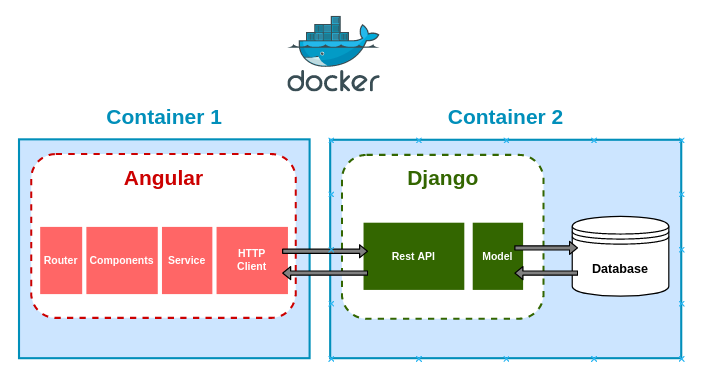
\includegraphics[width=\columnwidth]{./figures/architecture_with_docker}
	\caption{Überblick über die allgemeine Systemstruktur}
\end{figure}
\subsection{Randbedingungen und Risiken}
\section{Lösungsstrategie}
Architekturentscheidungen, -stile, -prinzipien, Vorgehen (z.B user centered design)
TODO:
\section{Fazit und Ausblick}




\begin{thebibliography}{00}
\bibitem{docker} \url{https://www.docker.com/}
\bibitem{angular} \url{https://angular.io/}
\bibitem{django} \url{https://www.django-rest-framework.org/}
\bibitem{mongodb} \url{https://www.mongodb.com/de}
\bibitem{docBox} \url{https://www.doctorbox.de/patienten.jsp}
\bibitem{notion} \url{https://www.notion.so/}
\end{thebibliography}
\end{document}
